\documentclass[10pt,a4paper,titlepage]{book}
\usepackage[russian]{babel}
\documentclass[10pt,a4paper,titlepage]{book}
%\documentclass[12pt,b5paper,titlepage]{book}
%\documentclass[10pt,a4paper,titlepage,twocolumn]{book}
\usepackage[utf8]{inputenc}
\usepackage{cmap}
\usepackage[ukrainian]{babel}
\usepackage[OT1]{fontenc}
\usepackage{amsmath}
\usepackage{amsfonts}
\usepackage{amssymb}
\usepackage{amsthm}
\usepackage{graphicx}
\usepackage{indentfirst}
\usepackage{bbm}
\usepackage{mathtools}
%\usepackage{index}
\usepackage{makeidx}
%\usepackage{showidx} % Show indeces on pages
\usepackage[
    unicode=true,
    breaklinks,
    colorlinks=true,
    linkcolor=blue,
    ]{hyperref}
\usepackage{enumitem}
\usepackage{verbatim}
\usepackage{framed}
\usepackage{pstricks}
\usepackage{cancel} % formulas cancel
\usepackage{multicol}
\author{Завадська Л.О., Савчук М.М.}

\pdfcompresslevel=9

\everymath{\displaystyle}

\theoremstyle{plain}
%\newtheorem{affirmation}{Утверждение}[section]
\newtheorem{theorem}{Теорема}[chapter]
%\newtheorem{lemma}{Лемма}[section]
\newtheorem{remark}{Зауваження}

\theoremstyle{definition}
\newtheorem{definition}{Визначення}[chapter]
\newtheorem{example}{Приклад}[chapter]

\theoremstyle{remark}

%\newcommand{\stcomp}[1]{{#1'}}
\newcommand{\stcomp}[1]{\overline{#1}}
\newcommand{\Probability}[1]{\mathbb{P}\left\{ #1 \right\}}
\newcommand{\probability}[1]{\mathbb{P}\left( #1 \right)}
\newcommand{\probabilityn}[1]{\mathbb{P}_n\left( #1 \right)}
\newcommand{\indicator}[1]{\mathbbm{1}\left( #1 \right)}
\newcommand{\Indicator}[1]{\mathbbm{1}\left\{ #1 \right\}}
\newcommand{\indicatorof}[1]{\mathbbm{1}_{#1}}
\newcommand{\meanof}[2]{M_{#1} #2}
\newcommand{\dispersionof}[2]{D_{#1} #2}
\newcommand{\dispersion}[1]{\dispersionof{}{#1}}
\newcommand{\mean}[1]{\meanof{}{#1}}
\newcommand{\covergence}[1]{\xrightarrow[n\to\infty]{#1}}
\newcommand{\Covergence}[1]{\xRightarrow[n\to\infty]{#1}}
\newcommand{\covergencen}[2]{\xrightarrow[#1\to\infty]{#2}}
\def \probabilityCovergenceText {\mathbb{P}}
\newcommand{\pcovergence}{\covergence{\probabilityCovergenceText}}
\newcommand{\pCovergence}{\Covergence{\probabilityCovergenceText}}
\def \almostSureCovergenceText {a.s.}
\newcommand{\acovergence}{\covergence{\almostSureCovergenceText}}
\newcommand{\aCovergence}{\Covergence{\almostSureCovergenceText}}
\def \distributionCovergenceText {d}
\newcommand{\dcovergence}{\covergence{\distributionCovergenceText}}
\newcommand{\dCovergence}{\Covergence{}}
\newcommand{\cdfof}[2]{F_{#1}\left(#2\right)}
\newcommand{\cdf}[1]{\cdfof{}{#1}}
\newcommand{\cdfn}[1]{F_n\left(#1\right)}
\newcommand{\CDFOF}[2]{F_{#1}\left\{#2\right\}}
\newcommand{\CDF}[1]{\CDFOF{}{#1}}
\newcommand{\pdf}[1]{p\left(#1\right)}

\newcommand{\integralc}[4]{\int\limits_{#1}^{#2} #4 #3}
\newcommand{\integral}[4]{\integralc{#1}{#2}{d #3}{#4}}
\newcommand{\integralp}[4]{\integralc{#1}{#2}{\partial #3}{#4}}

\newcommand{\argmaxof}[2]{\underset{#2}{\operatorname{arg\,max}}#1}
\newcommand{\argmax}[1]{\argmaxof{#1}{}}

\renewcommand{\thefootnote}{\fnsymbol{footnote}} 

%\renewcommand{\thesection}{Лекція \arabic{section}}
%\usepackage{titlesec}
%\titleformat{\section}{\normalfont\bfseries}{\thesection}{0.5em}{}
%\titleformat{\subsection}{\itshape}{}{0.5em}{}
%\titleformat{\subsection}{\normalfont\textit}{\thesubsection}{0.5em}{}

\pagestyle{empty} % Empty page header

\author{Савчук М.Н.}

\theoremstyle{plain}
\newtheorem{affirmation}{Утверждение}[section]
\newtheorem{theorem}{Теорема}[chapter]
%\newtheorem{lemma}{Лемма}[section]
\newtheorem{remark}[theorem]{Замечание}

\theoremstyle{definition}
\newtheorem{definition}[theorem]{Определение}
\newtheorem{example}[theorem]{Пример}

\title{Специальные разделы криптологии}

\makeindex
\begin{document}

\maketitle

\chapter{Алгоритм Шора для факторизации}

\chapter{Задача о скрытой подгруппе}

\chapter{Современные хэш-функции}

\section{Подходы к построению сжимающей функции}

Сжимающие функции современных хэш-функций строятся:

\begin{itemize}
  \item при помощи блочных шифров (см. ниже)
  \item при помощи поточных шифров --- в первую очередь, из-за скорости
  работы; обычно состояние хэша отождествляется с состоянием поточного
  шифра
  \item при помощи алгебраических операций (modular hashing) --- вызвано
  массовым распостранением аппаратуры, заточенной под RSA, и,
  соответственно, доступностью умножения и возведения в степень по
  модулю
  \item на NP-задачах (задачи на решётках, задачи укладки рюкзака \ldots)
  \item при помощи всякой экзотики (динамических хаос, клеточные
  автоматы, \ldots) \\[0.3cm]
\end{itemize}

\subsection{Схемы на основе блочных шифров}
Рассмотрим блочный шифр
\[ E: \{0,1\}^{m} \times \mathcal{K} \rightarrow \{0,1\}^{m} \]
\[Y = E_{k}(X)\]
\subsubsection{Функция Матяша-Мейера-Озиса (Matyas-Meyer-Oseas)}
\[H_{i} = E_{k(H_{i-1})}(X_{i}) \oplus X_{i}\]
тут $k(H_{i})$ --- преобразование блока $H_{i}$ в ключ шифрования \\[0.1cm]

Считается, что эта функция необратима, но это не доказано. Более того,
непонятно даже, какие требования нужно выдвигать к шифру $E$, чтобы
достигалась стойкость.

Однако Пренель доказал, что можно построить 12 сжимающих функций,
эквивалентных по стойкости функции ММО. Две главные из них:

\begin{description}
  \item[Функция Дэвиса-Мейера (Davis-Mayer)] \hfill \\
  $H_{i} = E_{k(X_{i})}(H_{i-1}) \oplus H_{i-1}$
  \item[Функция Миягути-Пренеля (Miyaguchi-Preneel)] \hfill \\
  $H_{i} = E_{k(H_{i-1})}(X_{i}) \oplus X_{i} \oplus H_{i-1}$
\end{description}

Все указанные функции неявно предполагают, что n = m = $\omega$, т.е., что
размеры блока, состояния и хэша совпадают. Однако размеры блоков современных
шифров (64 и 128 бит) недостаточны для обеспечения стойкости хэш-функции
к атакам общего вида.

Чтобы повысить стойкость и увеличить длину хэша по отношению к размеру
блока шифра, используют более навороченные схемы.\\[0.3cm]

\subsubsection{Функция MDC-2}
--- разработана Брахтом(Bracht), носит также название функции Мейера-Шиллинга
(Meyer-Shilling)\\
--- включена в ISO/IEC 10118-2 как рекомендованная схема

Функция сжатия в MDC-2 имеет вид:\\[0.3cm]
\[(H_{i},\widetilde{H}_{i}) = f(H_{i-1},\widetilde{H}_{i-1}, X_{i})\]
и использует 2 стартовых вектора $H_{0} = IV, \widetilde{H}_{0} = 
\widetilde{IV}$

Хэш-функция MDC-2 = схема MD + описанная функция сжатия.

Самая лучшая из известных атак на MDC-2 требует $O(2^{3m})$ операция для
поиска прообраза и $O(2^{m})$ для поиска коллизии.\footnote{m --- размер
блока шифра, а не хэша}


Однако собственно сжимающая функция в этом плане слабая: требуется
$O(2^{m})$ и $O(2^{m/2})$ операция соответственно.

Этой слабости лишена функция MDC-4, но она ещё более навороченная, 
использует 4 шифра за раунд и потому ещё медленнее.\\[0.5cm]

\subsection{Обобщения схемы Меркле-Дамгора}

Придумано множество вариантов схемы MD, которые убирают те или иные
конструктивные недостатки или защищают от некоторых атак. Рассмотрим
основные из них.

\subsubsection{Концепция wide-pipe ("широкого канала")}
Предложена Люксом (Lucks).

Идея проста: раз уж стойкость хэш-функции сводится к стойкости сжимающей
функции, необходимо сделать часть состояния хэша ненаблюдаемой: $\omega
\geq 2n$. Тогда поиск коллизии для сжимающей функции требует $O(2^{\omega / 2})
= O(2^{n})$ операций --- столько же, сколько и поиск прообраза. Канал
широкий, в конце резко сужается.

Функции с $\omega = n$ стали называть narrow-pipe ("узкий канал")

\subsubsection{Рандомизированное хэширование}
Превращает хэш-функцию в универсальную хэш-функцию. Используется дополнительный
параметр --- "соль" (salt), который должен быть случайным.
\[H_{0} = IV; r = random\]
\[H_{i} = f(H_{i-1}, X_{i} \oplus r), i = \overline{1,t} \]
\[h(X) = (g(H_{t}), r) \]
Рандомизация помогает защититься от атак на основе предвычислений (атаки
компромисса), поскольку значение функции от одинаковых входов будет
всякий раз разное. Стойкость сильно зависит от стойкости используемого ГСЧ.

\subsubsection{Схема HAIFA (HAsh Iterated FrAmework)}
На каждом шаге используется 2 дополнительных параметра:

$s$ --- salt, обеспечивает параметризацию (или рандомизацию); если параметризация
не нужна, то $s$ = 0;

$l_{i}$ --- длина той части входного сообщения, которая обработана на данный
момент, включая блок $X_{i}$ (но без учёта паддинга)

Соответственно,
\[ H_{i} = f(H_{i - 1}, X_{i}, s, l_{i}) \]
Такое простое изменение резко усложнит поиск коллизий за счёт уникальности
обработки каждого блока данных $X_{i}$ в зависимости от позиции i. 
\footnote{Аналогия с полиалфавитными шифрами} Недостаток --- потеря в
вычислительной эффективности (f большого размера и, соответственно, её
вычисление требует больших ресурсов).

На схеме HAIFA построены хэш-функции Blake (финалист SHA-3) и "Стрибог"
(стандарт РФ)

\subsubsection{Хэш-функция Skein}
Один из финалистов конкурса SHA-3, отличается дерзким дизайном :)
\begin{itemize}
  \item используется специально разработанный шифр TreeFish
  \item ARX-дизайн: в вычислениях используються только сложение, xor и
  циклические сдвиги, что приводит к бешенной скорости работы
  \item заточка под 64-битную архитектуру
  \item narrow-pipe (в отличие от всех прочих финалистов SHA-3)
  \item специальный режим работы блочного шифра для хэширования
\end{itemize}

\paragraph{Режим UBI (Unique Block Iteration)}

Главная цель как в и HAIFA --- сделать сжатие каждого блока как можно 
более уникальным
\[H_{i} = E_{k(H_{i-1})}(format(x_{i}, cfg))\]
тут format --- функция форматирования входных данных в битовый блок по размеру входа шифра\\
cfg --- служебные данные, которые включают в себя:
\begin{itemize}
  \item длину обработанного сообщения в байтах(на данный момент)
  \item флаг "это первый блок" (1 бит)
  \item флаг "это последний блок" (1 бит)
  \item флаг "bitpad" (1 бит) --- использовалось ли выравнивание в битах
  \item идентификатор типа хэша (примерно равно salt)
  \item и всё, что пожелает разработчик
\end{itemize}

\subsubsection{Схема Gr{\o}stl}
Хэш-функция Gr{\o}stl --- тоже финалист SHA-3
\begin{itemize}
  \item радикальный wide-pipe
  \item отказ от использования шифров как более уязвимых к атакам на основе неподвижных точек и rebound-атак
\end{itemize}

Внутреннее состояние $\omega \geq 2n$; pad(X) включает длину сообщения.\\
Длина блока сообщения $m = \omega$; используются две перестановки P и Q над $\{0, 1\}^\omega$, которые должны быть "существенно различны"

$H_0 = IV(n)$ (стартовый вектор содержит длину хэша)\\
$H_i = f(H_{i - 1}, X_i), i = \overline{1, t}$\\
$f(h, m) = P(h \oplus m) \oplus Q(m) \oplus h$\\
$h(x) = g(H_t)$\\
$g(h) = trunc_n(P(h) \oplus h)$

Из всех финалистов SHA-3 Gr{\o}stl --- самая консервативная (и надёжная в этом плане)
хэш-функция. Недостаток --- и самая медленная, поскольку требуеются две огромные
перестановки (в самом Gr{\o}stl они реализованы на AES-подобных преобразованиях).

Новый украинский стандарт хэш-функции ДСТУ 7564:2014 ("Купина") построен на схеме Gr{\o}stl\\[0.4cm]

{\large{\bfseries Схема Sponge ("губка")}}\\[0.2cm]

На схеме Sponge основан алгоритм Кессак --- победитель SHA-3
\begin{itemize}
  \item полный отказ от всех существовавших архитектурных решений
  \item ориентация на битовые архитектуры
  \item wide-pipe
  \item использование только простых преобразований (без S-блоков)
  \item переменная длина генерируемого хэша (потенциально до бесконечности)
  \item не требует включения длины сообщения во входной поток (pad)
\end{itemize}

Состояние H разбивается на две части: R (rate --- "такса") --- m бит, и C (capacity --- "ёмкость") --- c бит; $\omega = m + c$

\[H_0 = R_0 || C_0 = 0^\omega\]
\[H_i = R_i || C_i = f(R_{i-1} \oplus X_i || C_i), i = \overline{1, t}\]
\[Z_{i - t} = R_i - 1\]
\[R_i || C_i = f(R_{i - 1} || C_{i - 1})\]
\[h(X) = trunc_n(Z_1 || Z_2 || \ldots )\]

Свойства:

\begin{itemize}
  \item Для Sponge используется фиксированная перестановка f над $\{0, 1\}^\omega$.
В силу сложности построения такой перестановки $\omega$ обычно тоже фиксируют
  \item Чем больше m, тем больше хэш; чем больше C, теб он надёжнее. Разработчики рекомендуют брать $c = 2n$ и $m = \omega - c$.
\footnote{в Keccak $\omega = 1600, c = 2n$, где $n = 128 \ldots 512$}
  \item Единственное требование к паддингу --- входной поток не должен заканчиваться
на серию нулей (иначе, как видно из схемы, возможны атаки на основе удлинения сообщений).
Поэтому разработчики предложили sponge-padding вида pad$(X) = 10\ldots01$
\end{itemize}

Поскольку Sponge генерирует хэш переменной длины, то очевидно, что стандартные методы оценивания стойкости к атакам общего вида (поиск прообраза, дни рождения и т.д.) не подходят
Оказывается, для Sponge параметром стойкости является не длина хэша, а ёмкость.


\newtheorem*{thm}{Теорема}


\begin{thm}
Для Sponge атаки общего вида требуют:\\
--- $O(2^c)$ операций для поиска (второго) прообраза\\
--- $O(2^{c/2})$ операций для поиска коллизии
\end{thm}

Показано, что стойкость Sponge сводится к сложности решения задачи CICO (constrained input, constrained output):\\
пусть $f: \{0, 1\}^N \rightarrow \{0, 1\}^N$ --- биекция, и $X, Y \subseteq\{0,1\}^N$;\\
требуется определить, существует ли $x \in X$ такой, что $f(x) \in Y$.

В общем случае эта задача считается сложной ($\in$ NP). Перестановка f должна выбираться с учётом требования стойкости к этой задаче.




\chapter{Коды аутентичности сообщений}

\chapter[Математическая теория кодов аутентификации]{Математическая
теория кодов аутентификации}
Сюда мы включаем и цифровые подписи и коды–имитовставки.
Стойкость кодов аутентификации базируется на:

\begin{itemize}
\item вычислительной стойкости (это очень очень сложно)
\item доказуемая стойкость (сведение к признанно сложной задаче)
\item безусловная стойкость (недостаточно информации для взлома)
\end{itemize}
Участники процесса аутентификации:

\begin{itemize}
\item отправитель $A$ (Алиса)
\item получатель $B$ (Боб) ($A$ и $B$ могут быть одним лицом)
\item криптоаналитик $Kr$ (Крамер) 
\item арбитр $Ar$ (Арнольд) (требуется в некоторых случаях)
\end{itemize}
\section{Построение кода аутентификации ($A$-кода)
(математическая модель)}

Пусть $S$ --- источник информации, который наблюдается $A$.

$S=\left\{{s}_{i} \mid i=1{\dots}\left|S\right|\right\}$  --–  эти сообщения
надо передать с аутентификацией

$M=\left\{{m}_{i} \mid i=1{\dots}\left|\text{М}\right|\right\}$ –-- множество
сообщений, полученных в результате кодирования

$E=\left\{{e}_{i} \mid i=1{\dots}\left|E\right|\right\}$ --– множество
алгоритмов кодирования с аутентификацией: 
${\forall}i:{e}_{i}:S\rightarrow M$

На все  ${e}_{i}$ распространяются такие условия:
\begin{enumerate}
\item\label{it:properties:e:inj}
  ${e}_{i}$ --- инъекция, однако может быть многозначной (в этом
  случае инъективность понимается в том смысле, что образы различных
  входов не пересекаются).
  Будем считать, что  $M=\bigcup\limits_{e \in E} e\left( S \right)$
  --– объединение $e\left( S \right)$
\item\label{it:properties:e:inv}
  Существет обратное отображение.
  Для  ${\forall}e \in S$ определим обратное отображение
  \begin{equation*}
    {f}_{e}:M\rightarrow S \cup \left\{ 0 \right\}
  \end{equation*}
  То есть
  \begin{equation*}
    \begin{cases}
      \forall s \in S, e \in E&: {f}_{e}\left(e\left(s\right)\right)=S,\\
      \forall m \notin e\left( S \right)&: {f}_{e}\left(m\right)=0.
    \end{cases}
  \end{equation*}
\end{enumerate}


\begin{example}
  Если $e$ –-- алгоритм шифрования с ключом $K$, то  ${f}_{e} = ?$
  --- алгоритм шифрования на том же ключе.
\end{example}

Код аутентификации --– тройка $AK = <S, E, M>$, где 
\begin{itemize}
  \item
    $S$ --- множество сообщений (открытых текстов) = состояний источника
сообщений
  \item
    $E$ --– множество кодов $e:S\rightarrow M$
  \item
    $M$ --– множество сообщений для передачи (закодированных сообщений) и
    выполняются условия \ref{it:properties:e:inj} и \ref{it:properties:e:inv}
    для отображений $e$
\end{itemize}

 Свойства:

\begin{itemize}
  \item
    Множество кодов $E$ --- открытая информация и известна аналитику
  \item
    $A$ и $B$ предварительно строят $A$-код и выбирают из множества $E$
    случайное отображение для работы --- и выбранное отображение является
    секретом (общим секретом $A$ и $B$)
  \item
    Для передачи информации о состоянии источника $S$ $A$ вычисляет 
    $m = e\left( s \right)$ --– сообщение с аутентификацией; $m$ передается $B$
  \item
    Критерий аутентичности сообщения, который применяет $B$:

    ${f}_{e}\left(m\right){\neq}0$ --- сообщение подлинно

    ${f}_{e}\left(m\right)=0$ --- сообщение не подтверждено
\end{itemize}

Дополнительные свойства

\begin{itemize}
  \item
    $\left|M\right|{\geq}\left|S\right|$ (из инъективности)
  \item 
    если $\left|M\right|=\left|S\right|$, то 
    \begin{equation*}
       \left(\forall m \in M\right) \left(\forall e \in E\right)
       \left(\nexists s \in S\right): e\left(s\right)=m
    \end{equation*}
    по сути это приведёт к тому, что все сообщения будут аутентичними и
    сама схема не пройдет
  \item
    $\left|M\right|>\left|S\right|$ (обычно даже
    $\left|M\right|{\gg}\left|S\right|$)
  \item
    Пусть
    \begin{equation*}
      E\left( m \right)
      = \left\{e \mid m \in e\left(S\right)\right\}
      =\left\{e \mid \exists s:e\left(s\right)
      =m\right\}
    \end{equation*}

    Если  $\left|E(m)\right|=1$, то всё, аналитик сразу нашел правильное $e$
    $\Rightarrow $ всё взломано.
    Отсюда новое условие на $A$-код: 
    ${\forall}m:\left|E\left(m\right)\right|>1$.

    С другой стороны, если  $\left|E\left(m\right)\right|=\left|E\right|$,
    то любое сообщение подойдет как правильное, так как
    \begin{equation*}
      \left(\forall e\right)\left(\exists s\right):e\left(s\right)=m.
    \end{equation*}
    Криптоаналитик тогда может найти ложное сообщение из множества
    $\bigcap\limits_{e{\in}E}e\left( S \right)$ 
    Уточнение к написанному (и новое условие на $A$-код) 
    \begin{equation*}
      {\forall}m:\left|E\left( m \right)\right|<\left|E\right|
    \end{equation*}
  \item
    Если $\bigcap\limits_{e{\in}E\left( m \right)} e\left( S \right) > 1$,
    то аналитик всегда сможет подобрать ложные сообщения, которые будут
    трактоваться как правильные (подделка).
    Отсюда следует последнее, пятое условие на А-код:
    \begin{equation*}
      \bigcap\limits_{e{\in}E\left( m \right)}e\left( S \right)
      = \left\{ m \right\}
    \end{equation*}
\end{itemize}

\begin{example}
Если $e$ --- многозначная функция, то $A$-код называется кодом с расщеплением
(если однозначная, то код без расщепления).

Задать $A$-код можно матрицей  $\left|E\right|\times \left|M\right|$ ---
матрицей $A$-кода.

Пусть $S = \left\{ H, T \right\}$,
$M=\left\{{m}_{1},{m}_{2},{m}_{3},{m}_{4}\right\}$,
$E=\left\{{e}_{1},{e}_{2},{e}_{3},{e}_{4}\right\}$.

Расщепление: ${e}_{3}\left(H\right)=\left\{{m}_{2}, {m}_{3}\right\}$

\begin{center}
  \begin{tabular}{|*{5}{c|}}
    \hline
    \backslashbox{e}{m} & $m_1$ & $m_2$ & $m_3$ & $m_4$ \\
    \hline
    $e_1$               &  $H$  &  $T$  &  $0$  &  $0$  \\
    \hline              
    $e_2$               &  $H$  &  $0$  &  $T$  &  $0$  \\
    \hline              
    $e_3$               &  $0$  &  $H$  &  $H$  &  $T$  \\
    \hline              
    $e_4$               &  $0$  &  $0$  &  $T$  &  $H$  \\
    \hline
  \end{tabular}
\end{center}

Если в каком-то столбике будет только один символ (как в  ${m}_{1}$, то
это будет код без секрета --- аналитик узнает, какое было сообщение,
однако оно всё равно будет аутентифицировано. 

Проверим выполнение всех условий:

\begin{enumerate}
  \item
    Условие
    \begin{equation*}
      M=\bigcup\limits_{e}\left(S\right)
    \end{equation*}
    Проверим
    \begin{equation*}
      \begin{split}
        {e}_{1}\left(S\right)&=\left\{{m}_{1},{m}_{2}\right\} \\
        {e}_{2}\left(S\right)&=\left\{{m}_{1},{m}_{3}\right\} \\
        {e}_{3}\left(S\right)&=\left\{{m}_{2},{m}_{3},{m}_{4}\right\} \\
        {e}_{4}\left(S\right)&=\left\{{m}_{3},{m}_{4}\right\}
      \end{split}
    \end{equation*}
    выполняется.
  \item
    ${\forall}s:{f}_{e}\left(e\left(s\right)\right)=s$ --- выполняется
  по построению.
  \item
    $\left|M\right| > \left| S \right|$ --- выполняется.
  \item
    Условие
    \begin{equation*}
      {\forall}m:\left|E\right|>\left|E\left(m\right)\right|>1
    \end{equation*}
    Проверка
    \begin{equation*}
      \begin{split}
        E\left({m}_{1}\right)&=\left\{{e}_{1},{e}_{2}\right\} \\
        E\left({m}_{2}\right)&=\left\{{e}_{1},{e}_{3}\right\} \\
        E\left({m}_{3}\right)&=\left\{{e}_{2},{e}_{3},{e}_{4}\right\} \\
        E\left({m}_{4}\right)&=\left\{{e}_{3},{e}_{4}\right\} \\
      \end{split}
    \end{equation*}
    выполняется.
  \item
    Условие
    \begin{equation*}
      {\forall}m: \bigcap\limits_{e \in E\left( m \right)} e\left( S \right)
                  = \left\{m\right\}
    \end{equation*}
    Проверка
  \begin{equation*}
    \begin{split}
      &{m}_{1}:{e}_{1}\left(S\right) \cap {e}_{2}\left(S\right)
      =\left\{{m}_{1}\right\} \\
      &{m}_{2}:{e}_{1}\left(S\right) \cap {e}_{3}\left(S\right)
      =\left\{{m}_{2}\right\} \\
      &{m}_{3}:{e}_{2}\left(S\right) \cap {e}_{3}\left(S\right)
               \cap {e}_{4}\left(S\right)
      =\left\{{m}_{3}\right\} \\
      &{m}_{4}:{e}_{3}\left(S\right) \cap {e}_{4}\left(S\right)
      =\left\{{m}_{3},{m}_{4}\right\}
    \end{split}
    \end{equation*}
    не выполняется
  \end{enumerate}
\end{example}

\section{$A$-коды с аутентификатором,
  т.е. с добавочной информацией для аутентификации (имитовставки, цифровые
  подписи)}

\begin{figure}[h]
  \centering
  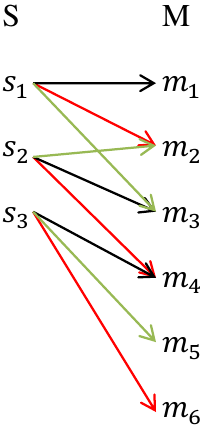
\includegraphics[scale=0.5]{a_codes}
\end{figure}
\begin{equation*}
  E = \left\{ {e}_{1},{e}_{2} \right\} \cup \left\{{e}_{3}\right\}
\end{equation*}
\begin{equation*}
{e}_{1}:\qquad
{s}_{1}\rightarrow {m}_{1},\qquad
{s}_{2}\rightarrow {m}_{3},\qquad
{s}_{3}\rightarrow {m}_{4} \qquad
\end{equation*}

\begin{equation*}
{e}_{2}:\qquad
{s}_{1}\rightarrow {m}_{3},\qquad
{s}_{2}\rightarrow {m}_{2},\qquad
{s}_{3}\rightarrow {m}_{5} \qquad
\end{equation*}

\begin{equation*}
{e}_{3}:\qquad
{s}_{1}\rightarrow {m}_{2},\qquad
{s}_{2}\rightarrow {m}_{4},\qquad
{s}_{3}\rightarrow {m}_{6} \qquad
\end{equation*}

Проверяем условия:
\begin{enumerate}
  \item
    \begin{equation*}
      M=\bigcup\limits_{e}e\left(S\right)
    \end{equation*}
    Не выполняется: ${m}_{6}$ не достижимо.

    \begin{equation*}
      {e}_{1}\left(S\right)=\left\{{m}_{1},{m}_{3},{m}_{4}\right\},\qquad
      {e}_{2}\left(S\right)=\left\{{m}_{2},{m}_{3},{m}_{5}\right\}
    \end{equation*}
    Но с ${e}_{3}$ будет выполняться: 
    \begin{equation*}
      {e}_{3}\left(S\right)=\left\{{m}_{2},{m}_{4},{m}_{6}\right\}
    \end{equation*}

  \item
    ${\forall}s:{f}_{e}\left(e\left(S\right)\right)=S$ --- выполняется

  \item
    $\left| M \right| > \left| S \right|$ --- таки да

  \item
    ${\forall}m:1<\left|E\left(m\right)\right|<\left|E\right|$

    $E\left({m}_{1}\right)=\left\{{e}_{1}\right\}$ --- очень плохо

    $E\left({m}_{2}\right)=\left\{{e}_{2},{e}_{3}\right\}$

    $E\left({m}_{3}\right)=\left\{{e}_{1},{e}_{2}\right\}$

    $E\left({m}_{4}\right)=\left\{{e}_{1},{e}_{3}\right\}$

    $E\left({m}_{5}\right)=\left\{{e}_{2}\right\}$ --- очень плохо

    $E\left({m}_{6}\right)=\left\{{e}_{3}\right\}$ --- очень плохо

    Если аналитик пронаблюдает  ${m}_{1}$, ${m}_{5}$, ${m}_{6}$ он будет точно
    знать, что используется отображение  ${e}_{1}$,  ${e}_{2}$, или 
    ${e}_{3}$ соответственно (и узнаёт состояние, которое защищалось). 

    $\Rightarrow$ Легко сделать обман/подделку (потому что
    известно кодирующее отображение).

    Если же {\textbar}E(m){\textbar}={\textbar}E{\textbar} и m раньше
    не посылалось, то аналитик просто отправляет m Бобу, и тот его с
    радостью принимает, потому что какое бы ни использовалось кодирующее
    отображение, m будет правильным сообщением.

  \item
    $\forall m: \bigcap\limits_{e \in E\left( m \right)} e\left( S \right) = \left\{ m \right\}$
    не выполняется уже для $m_1$:

    \begin{equation*}
      \bigcap\limits_{e \in E\left( m \right)} e\left( S \right)
        = \left\{{m}_{1},{m}_{3},{m}_{4}\right\}
    \end{equation*}

    Аналитик ловит сообщение $m$ и обнаруживает, что

    \begin{equation*}
      \bigcap\limits_{e \in E\left( m \right)} e\left( S \right)
      = \left\{m,m'\right\} \Rightarrow m'
    \end{equation*}
    тоже будет правильным сообщением, хотя $e$ осталось неизвестным.
\end{enumerate}

! Для того, чтобы аналитик не смог подделать сообщение путём случайного
выбора, необходимо, чтобы 
${\forall}c:\left\{m:{f}_{e}\left(m\right)=0\right\}$ было большим.

В этом случае случайный выбор $m$ попадет на $0$ с большой вероятностью.

$A$-код без секретности --- не скрывает состояние $S$. 

В этом случае можно и представить его в виде $A$-кода с аутентификатором: 
 $M{\subseteq}S\times A$.

$m=(s, a)$, $a$ --- аутентификатор.

Пусть  $\overline{e}: S \rightarrow A$ --- функция вычисления аутентификатора.

\subsection{Построение $A$-кода с аутентификатором по $A$-коду без секретности}

Обозначим:

\begin{equation*}
  \begin{split}
    M\left(S\right)
      &=\left\{ m\in M\mid\exists e \in E:e\left(S\right)=m\right\} \\
    \mu_{s}
      &=\left|M\left(S\right)\right| \\
    \mu
      &=\max\limits_{s}{\mu}_{s}
  \end{split}
\end{equation*}
Зная $\mu$, выбираем произвольное множество 
$A = \left\{{a}_{1},{\dots},{a}_{\mu }\right\}$, которое будем
использовать в качестве аутентификаторов.

Новое множество сообщений  $M=\left\{{m}_{1},{\dots},{m}_{\gamma
}\right\}{\subseteq}S\times A$  ?

Тогда  $M\left(S\right)=\left\{{m}_{{i}_{1}},{\dots},{m}_{{i}_{{\mu
}_{s}}}\right\}$,  ${\mu }_{{i}_{j}}={e}_{j}(S)$  ?

Положим  $\overline{e_j\left( S \right)}={a}_{j}$,
$j=\overline{{1,{\dots},{\mu }_{s}}}$ и поставим взаимно-однозначное
соответствие: $M\left(S\right)\leftrightarrow {M}_{s}$

\begin{equation*}
  {M}_{s}
  =\left\{\left({s}_{1},{a}_{1}\right),
          \left({s}_{1}, {a}_{2}\right), {\dots},(s_1,{a}_{\mu_s})\right\}
\end{equation*}
Тогда новое множество сообщений $\overline{M}=\bigcup_s M_s$

\begin{example}
  \begin{equation*}
    S=\left\{H,T\right\},\qquad
    M=\left\{{m}_{1},{\dots},{m}_{5}\right\},\qquad
    E=\left\{{e}_{1},{\dots},{e}_{6}\right\}
  \end{equation*}

  \begin{center}
    \begin{tabular}{|*{6}{c|}}
      \hline
      \backslashbox{e}{m} & $m_1$ & $m_2$ & $m_3$ & $m_4$ & $m_5$ \\
      \hline
      $e_1$               &  $H$  &  $T$  &  $0$  &  $0$  & $0$   \\
      \hline              
      $e_2$               &  $0$  &  $0$  &  $H$  &  $T$  & $0$   \\
      \hline              
      $e_3$               &  $0$  &  $0$  &  $H$  &  $0$  & $T$   \\
      \hline              
      $e_4$               &  $H$  &  $0$  &  $0$  &  $T$  & $0$   \\
      \hline
      $e_5$               &  $0$  &  $T$  &  $H$  &  $0$  & $0$   \\
      \hline
      $e_6$               &  $H$  &  $0$  &  $0$  &  $0$  & $T$   \\
      \hline
    \end{tabular}
  \end{center}

  Секретности нет: каждое  ${m}_{i}$ получается либо только из Н, либо
  только из Т.

  \begin{equation*}
    \begin{split}
      M\left(H\right)&=\left\{{m}_{1},{m}_{3}\right\} \\
      M\left(T\right)&=\{{m}_{2},{m}_{4},{m}_{5}\} \\
      \mu&=3 \\
      {\mu }_{H}&=2 \\
      {\mu }_{T}&=3
    \end{split}
  \end{equation*}
   $A=\left\{{a}_{1},{a}_{2},{a}_{3}\right\}$ --- аутентификаторы
   $\left\{a,b,c\right\}$
  Тогда
  \begin{equation*}
    \begin{split}
      {M}_{H}&=\left\{\left(H,a\right),\left(H,b\right)\right\} \\
      {M}_{T}&=\{\left(T,a\right),\left(T,b\right),(T,c)\} \\
      \overline{M}&={M}_{H} \cup {M}_{T} \subseteq S\times A
    \end{split}
  \end{equation*}
  Отображение $M\rightarrow \overline{M}$:
  \begin{equation*}
    \begin{split}
    {m}_{1}\rightarrow \left(H,a\right),\qquad
    {m}_{2}\rightarrow \left(T,a\right),\qquad
    {m}_{3}\rightarrow \left(H,b\right),\\
    {m}_{4}\rightarrow \left(T,b\right),\qquad
    {m}_{5}\rightarrow \left(T,c\right).
    \end{split}
  \end{equation*}
\end{example}


\bibliographystyle{../utf8gost705u}
\bibliography{bibliography}
\printindex
\tableofcontents
\end{document}
